\section{Design}
\label{sec:design}

CuPath follows a memory request from the local cache hierarchy to HBM and,
when necessary, across the wafer. Each stage acts only on information that is
already visible at that point. The local L2 observes whether adjacent demand
misses repeatedly share one controller access region. Requester RDMA observes
duplicate remote lines and requests headed to the same owner and page. A
returned remote line reveals whether the line is likely to be used again.
CuPath turns these observations into three consecutive transformations shown
in Fig.~\ref{fig:cupath-overview}. Cuckoo-Filter-Guided Local Pairing adapts
local HBM accesses, Cuckoo-Filter-Guided Remote Aggregation combines requests
before network injection, and Cuckoo-Filter-Guided Remote Reuse retains data
only after recurrence becomes visible.

\subsection{Shared Typed Membership State}

CuPath places one typed Cuckoo Filter beside each L2 partition
\cite{fan2014cuckoo}. RDMA accesses the Filter selected by the request address,
so it does not require a separate RDMA-side Filter. The four L2 partitions in
each of the 48 GPMs therefore provide 192 physical Filters across the wafer.
One physical bucket array stores five kinds of lifecycle information.
\textsc{Resident} represents lines installed in the local L2,
\textsc{Remote-Pending} represents remote lines already tracked by requester
RDMA, and \textsc{Remote-Batch} represents a joinable batch for one process,
owner GPM, and page. \textsc{Seen} records a completed remote access that was
not retained, and \textsc{Pattern} represents real-demand-trained remote
prediction state.
The type is included in the key and separates the logical namespaces without
creating five physical arrays.

The Filter is an accelerator rather than an authoritative directory. A
reliable negative result proves that an exact structure need not be searched.
A positive result is only a possible match and is confirmed by an L2 tag,
MSHR, or RDMA line-table lookup. If an insertion fails or a metadata result is
not reliable, the request follows the conservative exact path. Filter access
uses modeled lookup and update ports. Local lookups begin while the demand is
passing through the ordinary L2 pipeline, and remote lookups begin while the
request is entering RDMA. The Filter latency therefore overlaps existing path
latency whenever its ports are available.

\subsection{Cuckoo-Filter-Guided Local Pairing}
\label{sec:design-m1}

Motivated by O2 and O3, Local Pairing combines adjacent local read misses that repeatedly
use the same row-local HBM region. In the baseline, each L2 read miss generates
an independent HBM request even when the adjacent cacheline is requested soon
afterward. Local Pairing keeps the cacheline and MSHR formats unchanged and modifies only
the read sent to HBM. Since the write-back L2 already absorbs and combines
writes, Local Pairing does not alter the write path. A write hit updates the cached line,
a full-line write miss avoids an HBM read, and a partial write miss merges with
the existing L2 MSHR and fill path.

Local Pairing adds a bounded pair detector to each L2 partition. For every real L2 read
miss, the detector records its aligned two-cacheline HBM region. A later demand
for the other cacheline provides positive evidence and increments a saturating
confidence counter. If the recorded relation repeatedly expires without the
other demand, the counter decreases. Only real demand misses train the
detector, so an extra line fetched by Local Pairing cannot recursively create another
request.

When a local L2 read miss arrives, Local Pairing first consults the pair detector. If no
relation has been learned, Local Pairing sends the original cacheline request to HBM
immediately and uses the miss to update the detector. If an earlier paired read
already covers the requested line, the demand joins that access. Local Pairing similarly
suppresses another request when the adjacent line is already in flight or
waiting in the staging buffer.

When the detector identifies a pair candidate, Local Pairing queries \textsc{Resident} for
the adjacent cacheline. A reliable negative result shows that the candidate is
not represented as resident, while a possible match triggers an exact L2-tag
lookup. An exact hit removes the candidate, and an exact miss permits the
paired read.

If the candidate survives the checks and the ordinary downstream resources
are available, Local Pairing sends one HBM read covering the demand and its adjacent
cacheline. Otherwise, the demand follows the original singleton path without
waiting. The controller services the read with its existing address mapping,
row buffer, and burst interface \cite{li2016exploring,amd_rama_hbm}; Local Pairing adds no
new HBM command.

The demanded cacheline completes through the normal L2 fill path. A demand for
the adjacent cacheline can join the read while it is in flight. If no such
demand has arrived, the returned adjacent line enters a bounded staging buffer
and may satisfy a later L2 miss. A consumed adjacent line reinforces the
learned pair, whereas an unused line reduces its confidence. The staging
buffer accepts only the unused half of an issued paired read and is not a
separately addressable cache level.

\begin{figure}[t]
  \centering
  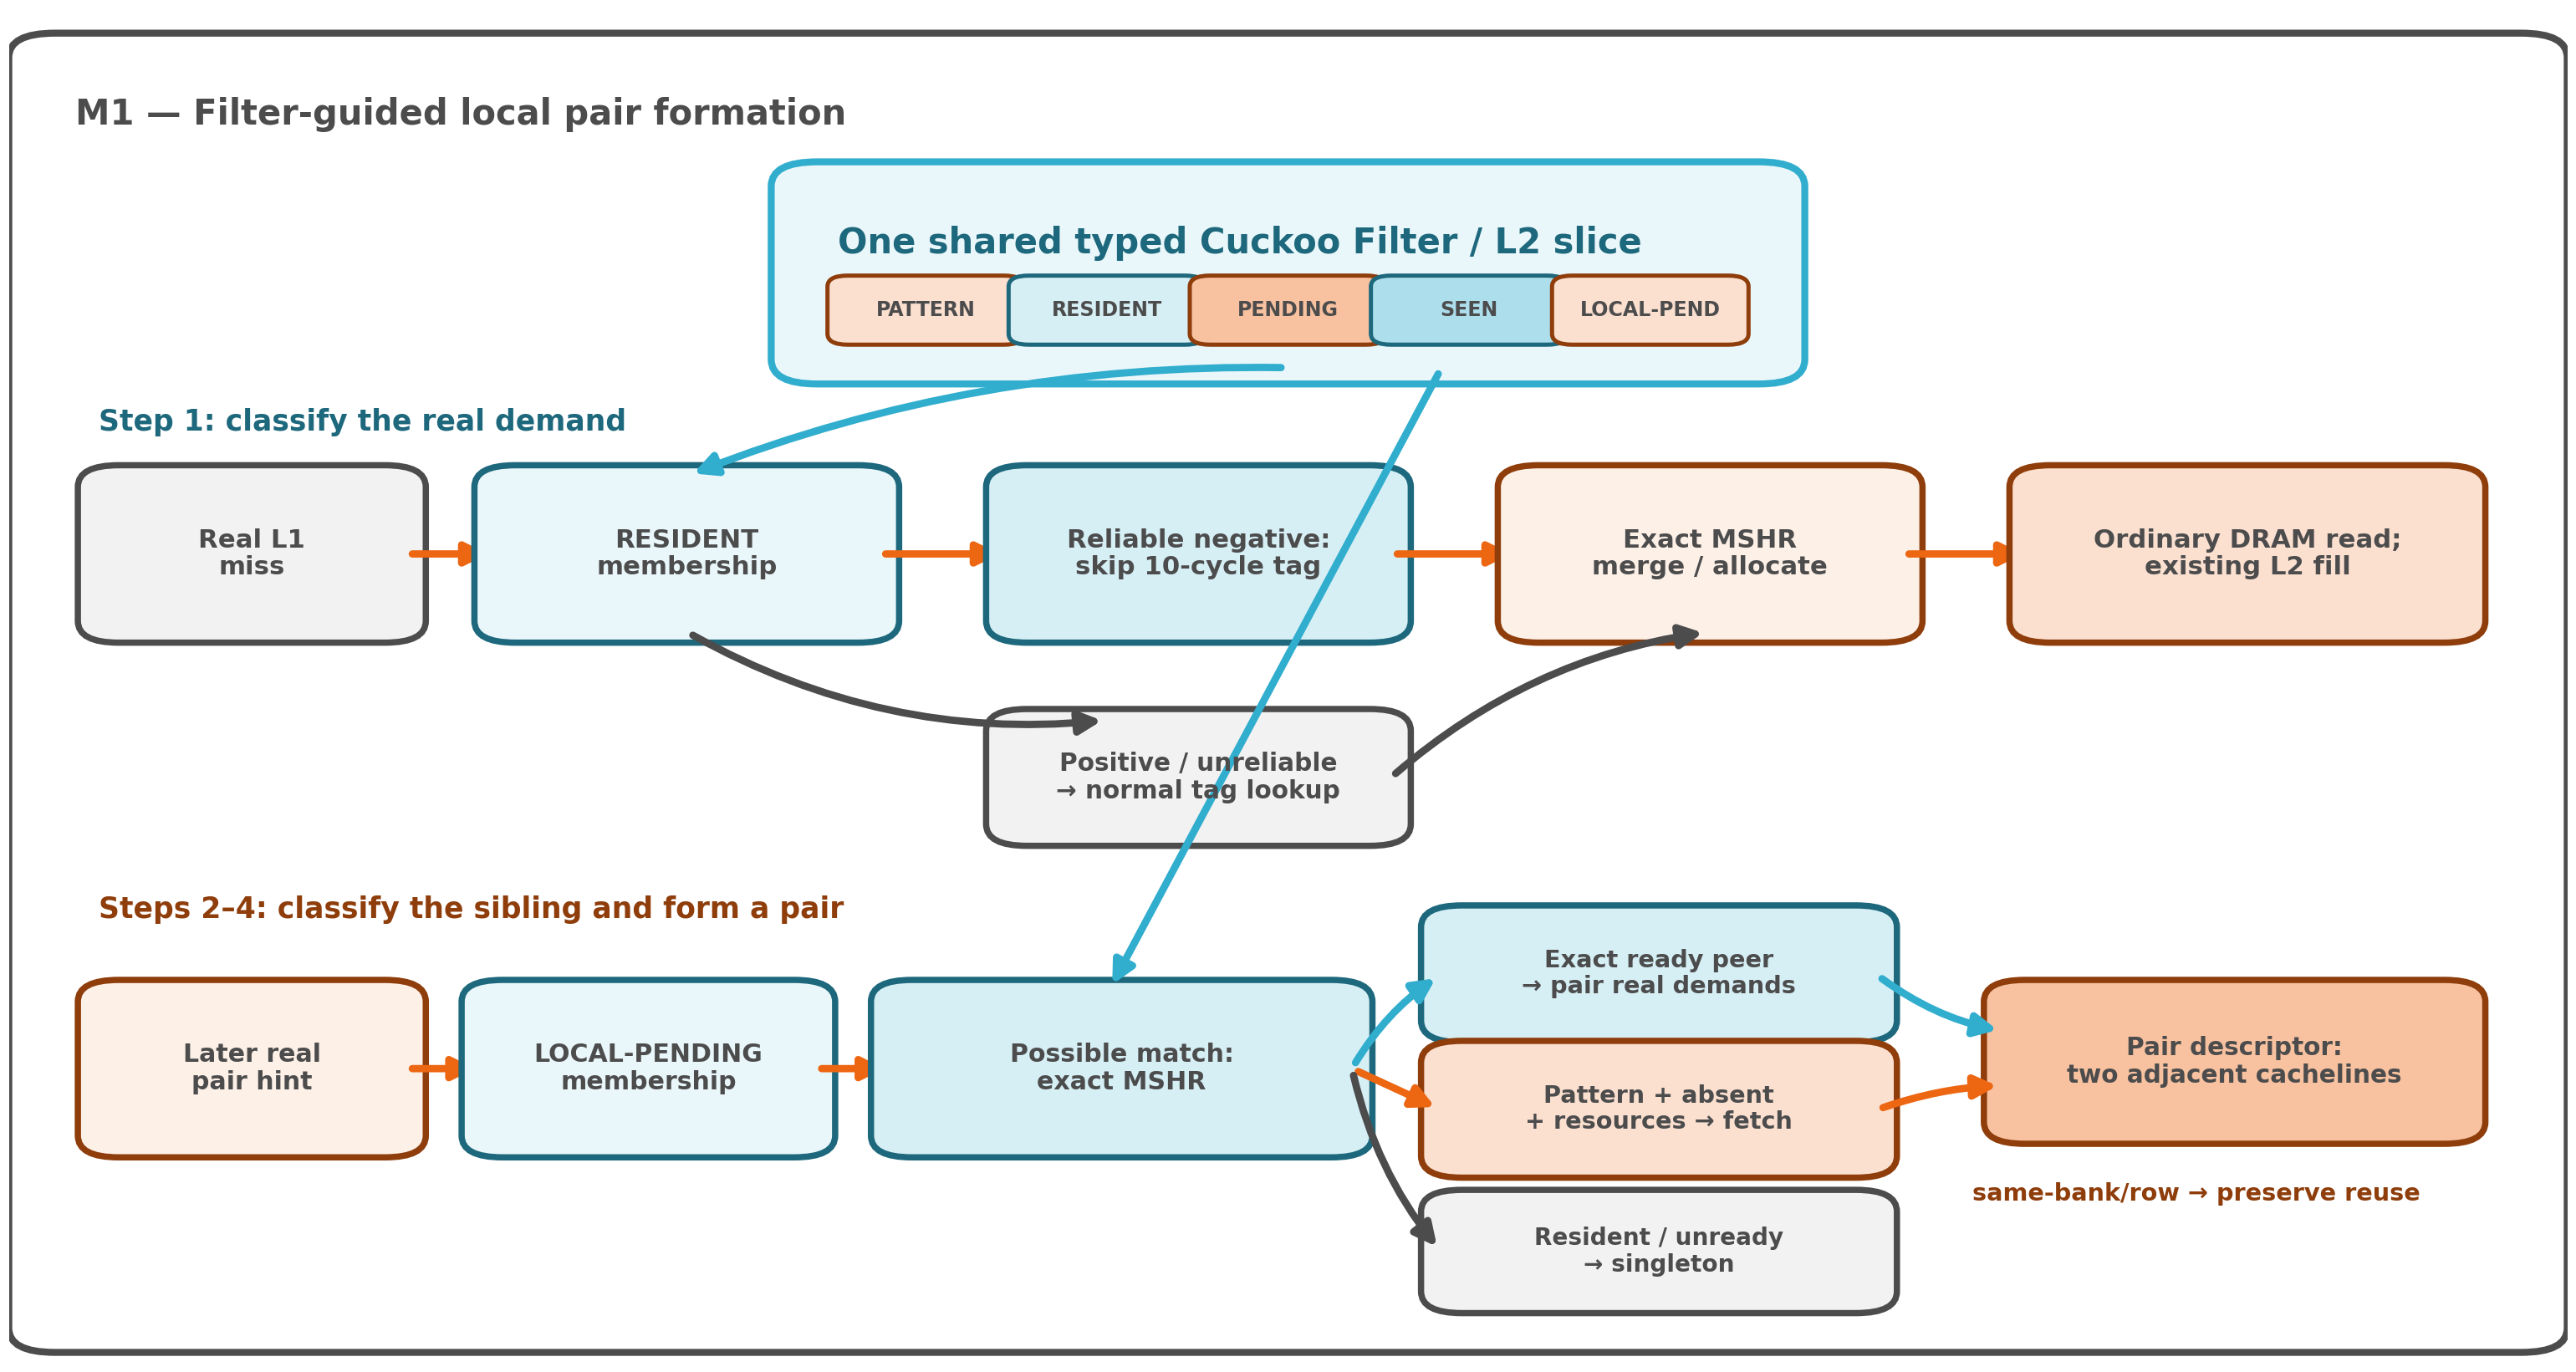
\includegraphics[width=\columnwidth]{Figure/M1.png}
  \caption{Local Pairing learns adjacent demand pairs, removes a line that is already
  resident or covered by an in-flight read, and otherwise fetches the pair
  with one HBM read.}
  \label{fig:cupath-m1}
\end{figure}

\subsection{Cuckoo-Filter-Guided Remote Aggregation}
\label{sec:design-m2}

Motivated by O4 and O5, Remote Aggregation combines remote requests before they consume
wafer-network work. Private L1 MSHRs cannot observe duplicate misses from
different L1 caches, while owner-L2 MSHRs act only after the requests have
crossed the wafer. Requester RDMA is the first point that observes all remote
misses from one GPM. Remote Aggregation uses the typed Cuckoo Filter at this point to identify
which requests may share existing work before consulting the exact RDMA state.
The Filter does not replace the request table or form packets by itself. It
guides both exact-line coalescing and the discovery of an active owner-page
batch, and prevents unnecessary lines from entering that batch.

For every issued remote line, Remote Aggregation inserts a \textsc{Remote-Pending} fingerprint
into the Filter. The exact requester-RDMA request table retains the complete
transaction, including its process, owner GPM, cacheline, write epoch, and
bounded waiter list. When another remote read arrives, Remote Aggregation first queries
\textsc{Remote-Pending}.

A reliable negative Filter result shows that no represented transaction is
outstanding for the line. Remote Aggregation therefore skips the exact same-line lookup,
allocates a new request-table entry, and inserts \textsc{Remote-Pending}. A
possible Filter match instead triggers an exact request-table lookup. If the
transaction exists, Remote Aggregation adds the demand to its waiter list, allowing one remote
operation to serve all matching L1 misses. A false positive simply allocates a
new entry and proceeds as a negative result.

A newly allocated line becomes the leader of a remote transaction. Remote Aggregation forms a
batch key from the process, owner GPM, and 4-KB page and queries
\textsc{Remote-Batch} before accessing the exact batch table.

A reliable negative Filter result shows that no joinable batch is represented
for the key. Remote Aggregation allocates a batch descriptor, records the leader in its bitmap,
and inserts \textsc{Remote-Batch}. A possible Filter match triggers an exact
batch-table lookup. The new leader joins a matching descriptor when a bitmap
position remains available. A false or stale match, or a full descriptor,
causes Remote Aggregation to allocate a new batch without delaying the request.

A batch remains represented by \textsc{Remote-Batch} only while at least one
matching descriptor can accept another line. When the last joinable descriptor
becomes full or is selected for egress, Remote Aggregation removes that state. A singleton is
sent as an ordinary remote read, while multiple leaders in one bitmap cross
the network as one packet. Owner RDMA expands the bitmap into ordinary
cacheline accesses to the existing owner L2. Returned lines are matched to
their exact request-table entries and fanned out to every waiting L1 request.
Remote Aggregation never delays a request to wait for a future partner and uses no batching
timeout.

The Filter also controls whether a predicted page-local line may use a free
position in an existing batch. \textsc{Pattern} must indicate a relation
trained by real remote demands, while reliable negative results for
\textsc{Resident} and \textsc{Remote-Pending} show that the line is neither
cached locally nor already in flight. \textsc{Remote-Batch} must also indicate
that a compatible batch may exist. Possible matches are confirmed using the
corresponding exact L2, request-table, predictor, and batch-table state. Remote Aggregation
admits the line only when the exact batch belongs to the same owner and page
and still has a free bitmap position. Otherwise, the candidate is discarded
without creating a packet or delaying a demand.

When the response completes, Remote Aggregation fans out the data, releases the exact request
entry, and deletes its \textsc{Remote-Pending} fingerprint. If a Filter result
or update is unavailable, Remote Aggregation uses the conservative exact path. Writes advance
the transaction epoch so that a read cannot merge with stale state. The Filter
therefore removes avoidable line-table and batch-table lookups, locates
possible aggregation opportunities, and filters predicted candidates. The
exact request table and bitmap batch remain authoritative.

\begin{figure}[t]
  \centering
  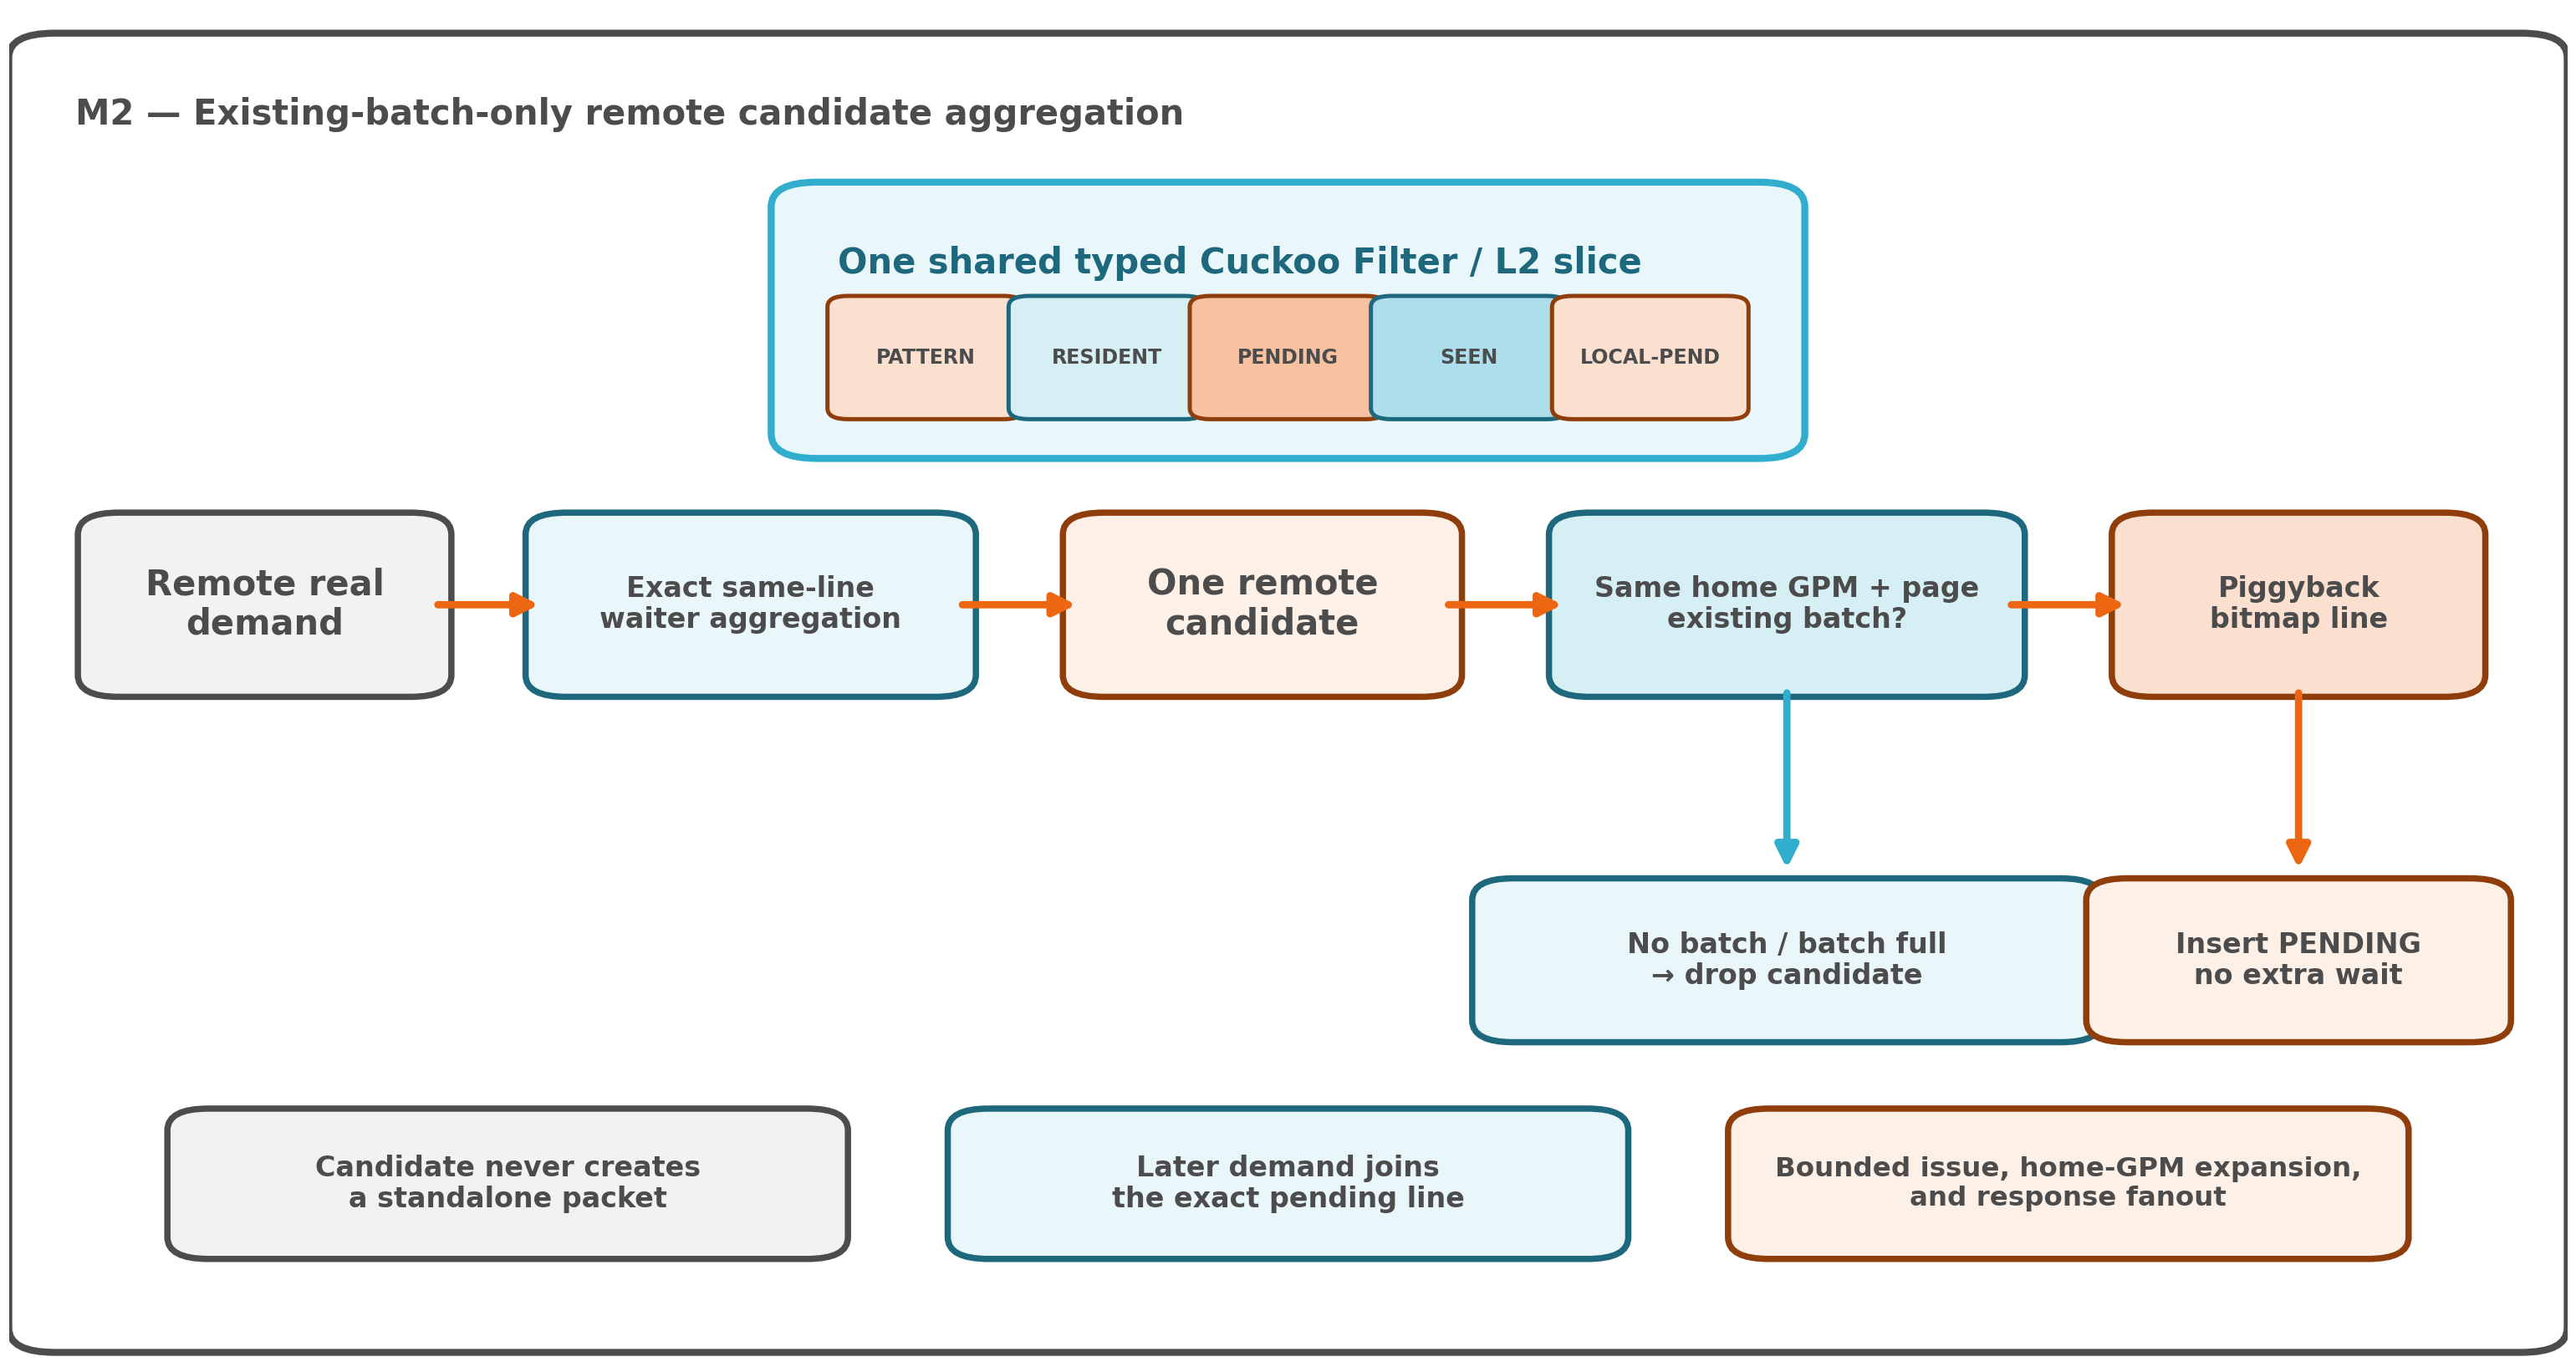
\includegraphics[width=\columnwidth]{Figure/M2.png}
  \caption{The typed Cuckoo Filter identifies possible in-flight duplicates,
  locates a joinable owner-page batch, and filters predicted candidates. Exact
  RDMA tables confirm matches before identical lines are merged or different
  lines are grouped into one packet.}
  \label{fig:cupath-m2}
\end{figure}

\subsection{Cuckoo-Filter-Guided Remote Reuse}
\label{sec:design-m3}

Motivated by O6, Remote Reuse uses the existing requester L2 to retain remote data only
after real accesses reveal reuse. The baseline sends a remote return directly
to requester L1. Once the line leaves L1, a later access repeats requester
RDMA, wafer-network, owner-L2, and possibly owner-HBM work. Filling every
remote return into requester L2 would avoid some traversals but would also
consume capacity for lines that never recur. Remote Reuse uses \textsc{Seen} to
distinguish recurring lines from one-time remote data and adds no new cache
level.

After requester RDMA finds no matching in-flight transaction, Remote Reuse checks
\textsc{Resident} and \textsc{Seen} before issuing the remote request.

Reliable negative results for both types identify a cold remote line that is
neither represented as resident nor previously observed. Remote Reuse bypasses the
otherwise guaranteed-miss requester-L2 tag lookup and sends the request to the
owner GPM. The first completed access returns to L1 without filling requester
L2 and inserts \textsc{Seen}. A possible Filter match indicates that the line
may be retained or recurring and triggers an exact requester-L2 tag lookup.
An L2 hit completes locally, while an exact miss follows the remote path and
preserves the reuse evidence for the returning response.

A response with real recurrence evidence becomes eligible for a clean fill in
requester L2. The second completed access supplies such evidence, and multiple
real demands merged by Remote Aggregation can establish it within one remote transaction. A
predicted line qualifies only if a real demand claims it while the transaction
is in flight. A successful fill updates \textsc{Resident}, allowing a later
access to complete locally without another wafer traversal.

Every fill remains best effort. Remote Reuse may use an invalid way or replace another
clean remote line, but it does not evict ordinary local data. A dirty, locked,
active-MSHR, or stale-generation victim rejects the fill. An unclaimed
predicted return can use only an invalid way. If a fill fails, \textsc{Seen}
remains recorded so that a later real access can try again. Remote writes
invalidate the corresponding reuse history and advance the exact transaction
epoch.

\begin{figure}[t]
  \centering
  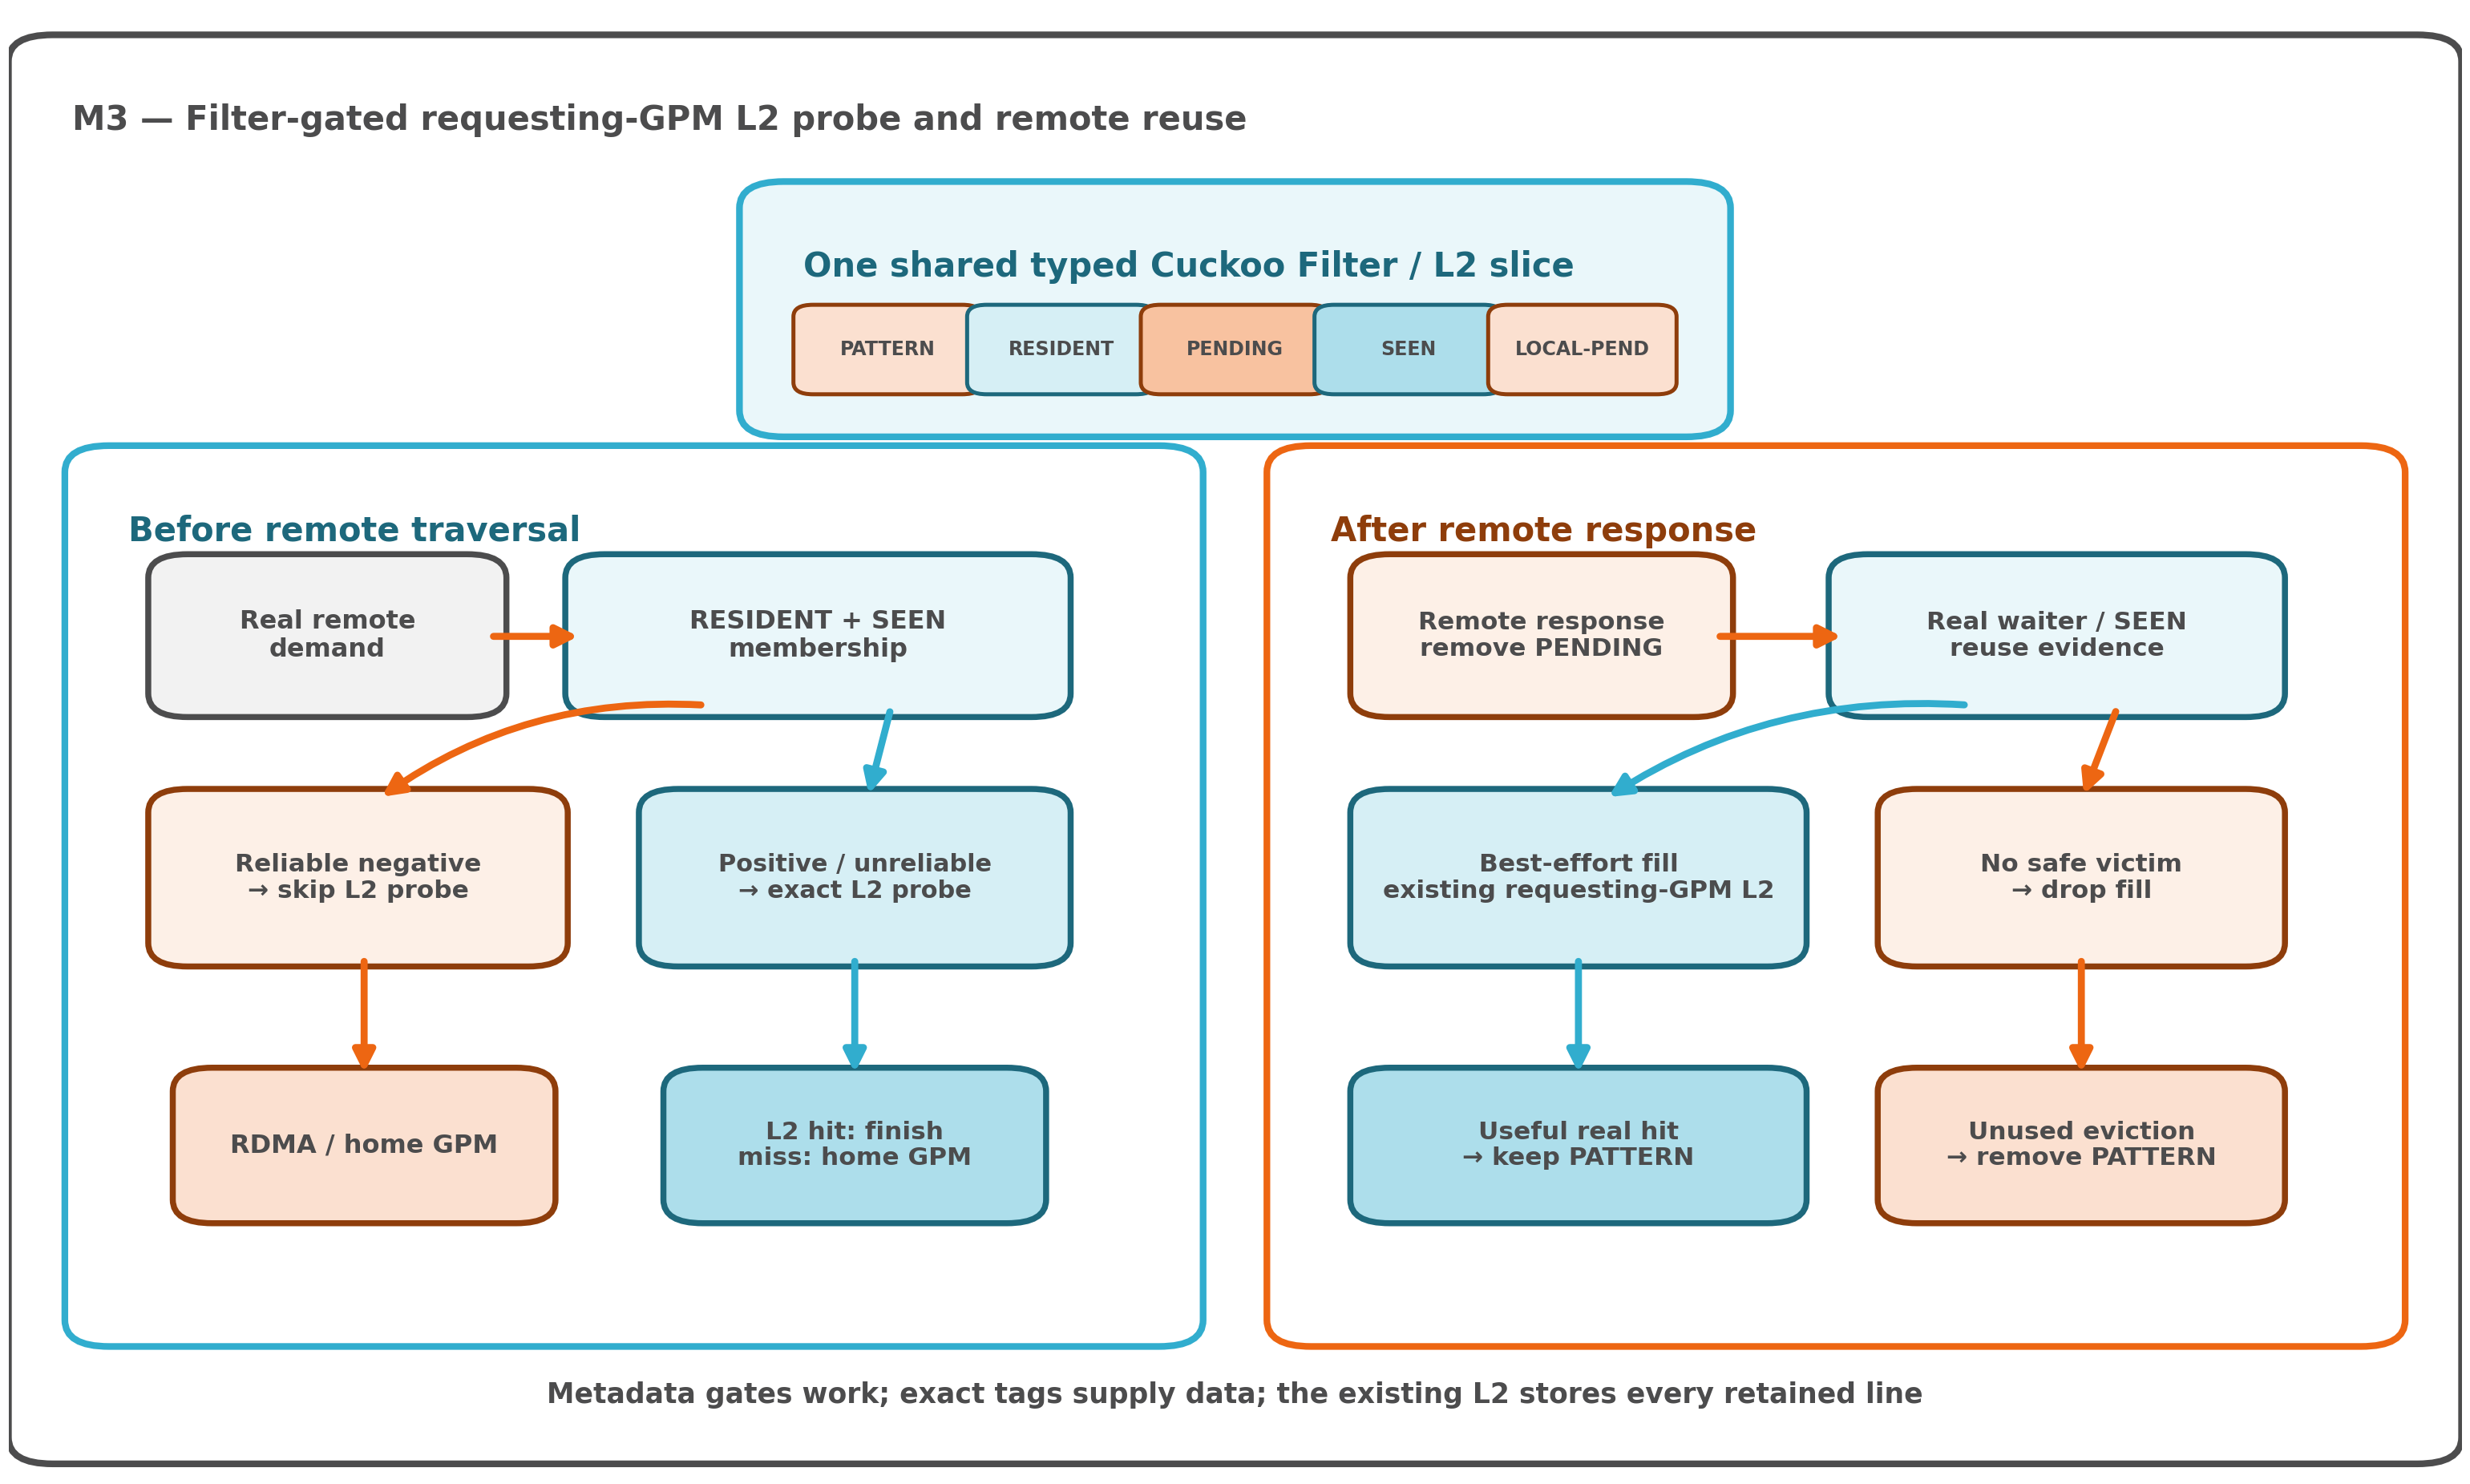
\includegraphics[width=\columnwidth]{Figure/M3.png}
  \caption{Remote Reuse bypasses known-miss requester-L2 lookups and retains a remote
  return in the existing requester L2 only after real accesses reveal reuse.}
  \label{fig:cupath-m3}
\end{figure}

\subsection{End-to-End Composition}

The three transformations operate on one request lifecycle. Local Pairing uses local demand
history and L2 residency to choose the amount of HBM work. Remote Aggregation uses global
request visibility and \textsc{Remote-Batch} state at requester RDMA to remove
duplicates and locate compatible network work. Remote Reuse uses completed remote
activity to decide whether another wafer traversal can be avoided. The typed
Cuckoo Filter carries compact lifecycle state between these decisions, while
exact structures preserve correctness. No mechanism waits for a speculative
opportunity. When evidence, metadata bandwidth, or downstream capacity is
unavailable, CuPath continues along the baseline path.
